\section{Polynomial port ranges and positive weights}\label{sec:ports}

The restricted Gaussian average in Lemma~\ref{lem:shift-average}
approximates $Z$ by a normalized weighted count of pairs of original
bases whose difference is supported on the representative edges. We now
describe these pairs by part totals and free edge coordinates. Only the
part totals will be discrete variables in the counting algorithm. The
free coordinates, whose ranges may depend on the numerical value of $R$,
will be integrated out. The resulting positive weights must satisfy the
two signatures of Definition~\ref{def:integer-signatures} at every
annealing power; this is the main purpose of the smoothing below.

\subsection{Part totals and an integral coordinate map}

For each $D\in\mathcal D_i$, define integer endpoints
\[
 L_{iD}=\max\{0,\lfloor c(D)-N^{20}W\rfloor\},\qquad
 U_{iD}=\min\{R,\lceil c(D)+N^{20}W\rceil\}.
\]
A \emph{port} is the part total $u_{iD}$, restricted to
$[L_{iD},U_{iD}]\cap\Z$. Its length
$d_{iD}=U_{iD}-L_{iD}$ is at most $N^{21}W$. Write
\[
 \bar r_i(\mathcal A)=r_i\left(\bigcup_{D\in\mathcal A}D\right),
 \qquad \mathcal A\subseteq\mathcal D_i.
\]
By Lemma~\ref{lem:base-calculus}, the projection of $B(r_i)$ onto its
part totals is $B(\bar r_i)$.

These ranges contain every term of the original restricted Gaussian
average, supported on representative edges, with
$|l_j|\le S/N^{25}$. Here is a quantitative justification. The center
property bounds the slack of every generator of $\mathcal D_i$ throughout
$P$ by $4(n+1)W$. The prefix construction in
Lemma~\ref{lem:generator-prefixes}, followed by subtraction of consecutive
prefix totals, therefore gives
\begin{equation}\label{eq:part-total-range}
 |x(D)-c(D)|\le N^{10}W\qquad(x\in P, D\in\mathcal D_i).
\end{equation}
Indeed there are at most $n^2$ generators and at most $n$ intersections
per prefix, so $8(n+1)n(n^2+1)W$ suffices. If
$x_1\in B(r_1)$, $x_2\in B(r_2)$, and
$x_1-x_2=d(l)$ with these bounds on $l$, then $x_1$ violates any
inequality of the second system by at most $\norm{d(l)}_1\le 2nS$.
Lemma~\ref{lem:polyhedral-controls} gives a point of $P$ within
$N^6S$ of $x_1$ in sup norm. The same assertion holds for $x_2$.
Consequently their part totals differ from $c(D)$ by at most
$N^{10}W+nN^6S<N^{20}W$. Nonnegativity and total rank put those totals
in $[0,R]$ as well.

Use the bipartite graph, component representatives $e_C$, and root
components $C_0(G)$ fixed in Section~\ref{sec:geometry}. For arbitrary
real port values, define
\begin{equation}\label{eq:component-imbalance}
 t_C(u)=\sum_{D\in C\cap\mathcal D_1}u_{1D}
       -\sum_{D\in C\cap\mathcal D_2}u_{2D}.
\end{equation}
Choose a spanning tree $\mathcal T_C$ in each component, containing
$e_C$. Let $z_e$, for edges outside these trees, be free coordinates.
We seek $X_1$ with side-1 margins $u_{1D}$ and side-2 margins $u_{2D}$,
except that $t_C$ is added to the side-2 margin incident to $e_C$.
The two margin sums in a component now agree. Define $X_2$ by
subtracting $t_C$ from $X_1$ on $e_C$, leaving all other edges unchanged.
Figure~\ref{fig:tree-ports} shows this correction and a free coordinate
in a component with one cycle.

\begin{lemma}[Integral tree coordinates]\label{lem:tree-coordinates}
There is a unique pair $X_i(u,z)$ with these properties and
$X_{1e}=z_e$ on nontree edges. Its coordinates are integral linear
functions of $(u,z)$, with coefficients of absolute value at most
$10(n+1)$. Each coordinate depends only on variables in its superblock.
For integral $(u,z)$ this is a bijection onto integral pairs with the
specified $\mathcal D_1$-totals for $X_1$ and $\mathcal D_2$-totals
for $X_2$, and with $X_1-X_2$ supported on the representatives.
\end{lemma}

\begin{proof}
Remove the prescribed nontree contributions from each vertex margin.
A leaf of the remaining tree determines its unique incident edge;
subtract that value from the neighboring margin and delete the leaf.
The final equation holds because the two margin sums agree. This proves
existence, uniqueness, and integrality. Equivalently, deleting a tree
edge divides the vertices into two sets; its value is the signed sum of
the residual margins on either one of those sets. Every original port
has coefficient $0$, $1$, or $-1$ in that sum before the representative
correction, and every free edge contributes with coefficient of absolute
value at most one. Substituting~\eqref{eq:component-imbalance} gives the
stated loose coefficient bound. Conversely, the prescribed margins of
any such pair give
$\sum_{e\in C}(X_{1e}-X_{2e})=t_C$.
Representative support forces its discrepancy on $e_C$ to equal
$t_C$, so it obeys exactly the equations just solved. The inverse map
reads off the part totals and nontree values. Thus there is no
multiplicity or lattice determinant in this parametrization.
\end{proof}

\begin{figure}[tb]
\centering
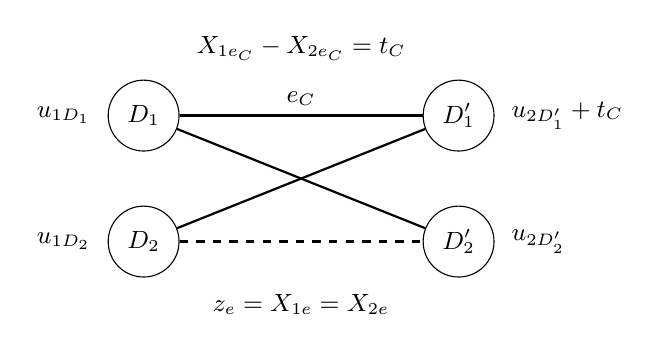
\begin{tikzpicture}[every node/.style={font=\small},
  vertex/.style={circle,draw,minimum size=9mm,inner sep=1pt}]
 \node[vertex] (a) at (0,1.6) {$D_1$};
 \node[vertex] (b) at (0,0) {$D_2$};
 \node[vertex] (c) at (4,1.6) {$D'_1$};
 \node[vertex] (d) at (4,0) {$D'_2$};
 \draw[thick] (a)--node[above] {$e_C$}(c);
 \draw[thick] (a)--(d);
 \draw[thick] (b)--(c);
 \draw[dashed,thick] (b)--(d);
 \node at (2,2.45) {$X_{1e_C}-X_{2e_C}=t_C$};
 \node at (2,-.8) {$z_e=X_{1e}=X_{2e}$};
 \node[anchor=east] at (-.55,1.6) {$u_{1D_1}$};
 \node[anchor=east] at (-.55,0) {$u_{1D_2}$};
 \node[anchor=west] at (4.55,1.6) {$u_{2D'_1}+t_C$};
 \node[anchor=west] at (4.55,0) {$u_{2D'_2}$};
\end{tikzpicture}
\caption{A schematic component with four edges. The solid edges form
the chosen tree; the dashed edge is a free coordinate. The displayed
right-hand margins are those for $X_1$. After solving the tree equations,
subtracting $t_C$ on $e_C$ gives the prescribed margins for $X_2$.
The construction applies to arbitrary bipartite multigraph components.}
\label{fig:tree-ports}
\end{figure}

Let $\mathcal F_G$ denote the nontree edges in a superblock $G$. In discrete sums
we take $z\in\{0,\ldots,R\}^{\mathcal F_G}$; for integration we use
$Q_G=[0,R+1]^{\mathcal F_G}$. These choices include every original base pair.
They also fix the measure: it is ordinary Lebesgue measure in $z$,
with a zero-dimensional integral equal to its integrand.

\subsection{Convex penalties and comparison with the count}

For each superblock $G$, let $A_{iG}$ be the union of blocks preceding
$G$ in the order for system $i$, with the reversed order for system 2.
Define the contracted ranks and their violation penalty by
\begin{align}
 r_{iG}(U)&=r_i(A_{iG}\cup U)-r_i(A_{iG})
       &&(U\subseteq G),\\
 V_G(u,z)&=\sum_{i=1}^2\max_{U\subseteq G}
                 \{X_i(u,z)(U)-r_{iG}(U)\},
 &\lambda&=N^{320}/W.\label{eq:block-penalty}
\end{align}
Each maximum includes the empty set, so $V_G$ is nonnegative and convex.
The hard conditions on ports are
\begin{equation}\label{eq:hard-port-conditions}
 u_i\in B(\bar r_i)\quad(i=1,2),\qquad
 \sum_{C\subseteq G}t_C=0\quad\hbox{for every }G.
\end{equation}

\begin{lemma}[What the penalties enforce]\label{lem:port-penalties}
An original base pair with a representative shift satisfies
\eqref{eq:hard-port-conditions} and $\sum_GV_G\le N^7S$.
Conversely, if~\eqref{eq:hard-port-conditions} holds, then
\[
 X_i(A)-r_i(A)\le\sum_G V_G\qquad(A\subseteq E, i=1,2).
\]
If in addition $\sum_GV_G\le T$, then $X_i\in B_i^+$ for both $i$,
where $B_i^+$ is defined in~\eqref{eq:expanded-bases}.
\end{lemma}

\begin{proof}
The representative shift has sum zero on each superblock, proving the
hard conditions. For an original pair, every forward superblock prefix $A$
satisfies $x_1(A)=x_2(A)$. Its two complementary rank slacks therefore
add to $s_*(A)\le N^4S$. The system-2 prefixes are complements of such
forward prefixes. In particular the slack at either prefix
$A_{iG}$ is at most $N^4S$. The inequality on $A_{iG}\cup U$ gives
\[
 x_i(U)-r_{iG}(U)\le r_i(A_{iG})-x_i(A_{iG}),
\]
so summing over the two systems and at most $n$ blocks proves the first
bound.

For the converse, fix $i$ and put $U_G=A\cap G$. Diminishing marginal
returns, applied successively in the order of system $i$, gives
\[
 \sum_G\bigl(r_i(A_{iG}\cup U_G)-r_i(A_{iG})\bigr)\le r_i(A).
\]
Indeed the prefix of the already selected pieces of $A$ is contained
in $A_{iG}$; its marginal increment from $U_G$ is at least the increment
from the full prefix. Summing the defining inequalities for $V_G$
proves the claim. The hard rank conditions enforce the correct total
and every inequality on a union of parts of $\mathcal D_i$. Any other
set cuts at least one part. Its rank bound in $B_i^+$ increases by
$T$ for every pair of coordinates in that part separated by the set,
and hence by at least $T$. This absorbs the remaining violation.
\end{proof}

Write $J=\sum_l\exp(-\sum_jl_j^2/M^2)$ for the normalizer of the
representative average of Lemma~\ref{lem:shift-average}. Consider
\begin{equation}\label{eq:discrete-port-sum}
 \mathcal A=\sum_{\substack{u\text{ in the integer port boxes}\\
                          \text{satisfying }\eqref{eq:hard-port-conditions}}}
 \ \sum_{z\in\{0,\ldots,R\}^{\bigcup_G\mathcal F_G}}
 \exp\left(-\lambda\sum_GV_G(u,z)
           -\sum_G\sum_{C\ne C_0(G)}t_C(u)^2/M^2\right).
\end{equation}
Under the hard block equality, the nonroot values $t_C$ are precisely
the independent representative star coordinates. Lemma~\ref{lem:tree-coordinates}
therefore identifies every summand with one representative-shift pair.
For a lower bound, retain original pairs with $|l_j|\le S/N^{25}$.
Their ports and free coordinates are in the chosen boxes, and their
additional penalty is at most
$\lambda N^7S=N^{327}S/W<N^{-20}$.
For an upper bound, the summands with $\sum_GV_G\le T$ form a subset
of the expanded representative average. The remaining summands have
total at most
\[
 e^K e^{-\lambda T}=\exp(K-N^{20}).
\]
The product bound associated with~\eqref{eq:scales} justifies $e^K$
here. Since $JZ\ge1$, this last bound is negligible also as a relative
error. Lemma~\ref{lem:shift-average} and
Proposition~\ref{prop:expansion} now give
\begin{equation}\label{eq:discrete-proxy-bound}
 \left|\log\frac{\mathcal A}{JZ}\right|\le40N^{-8}.
\end{equation}

Define the continuous block weights
\begin{equation}\label{eq:block-integral}
 I_G(u)=\int_{Q_G}\exp(-\lambda V_G(u,z))\dd z.
\end{equation}
They are positive. They are log concave by the theorem on marginals
of log-concave functions \cite{Prekopa1973}, applied to the integrand
times the indicator of its convex integration box. The tree coefficient
bound implies, globally in the joint variables $(u,z)$,
\begin{equation}\label{eq:port-lipschitz}
 |\lambda V_G(u,z)-\lambda V_G(u',z')|
 \le L_0\norm{(u,z)-(u',z')}_\infty,
 \qquad L_0=N^{330}/W.
\end{equation}
For example, at most $3n$ input variables, at most $n$ edge coordinates
per subset sum, and coefficients bounded by $10(n+1)$ give a Lipschitz
constant at most $100(n+1)^4\lambda<L_0$.
Integrating the corresponding pointwise ratio bounds proves the same
bound for $\log I_G$ in $u$. Define the hard integrated mass
\[
 \mathcal I_{\rm hard}
 =\sum_{\substack{u\text{ in the integer port boxes}\\
                    \text{satisfying }\eqref{eq:hard-port-conditions}}}
       \prod_G I_G(u)
       \exp\left(-\sum_G\sum_{C\ne C_0(G)}t_C(u)^2/M^2\right).
\]
Tiling $Q_G$ by unit cells anchored at
$\{0,\ldots,R\}^{\mathcal F_G}$ gives
\begin{equation}\label{eq:sum-integral-comparison}
 \left|\log\frac{\mathcal I_{\rm hard}}{\mathcal A}\right|\le2nL_0.
\end{equation}

\subsection{Smoothing and the paired count model}

We have obtained positive log-concave block integrals, but log concavity
alone does not imply either integer signature. We arrange a quantitative
version by smoothing on a scale on which the weights barely change,
then adding a smaller strictly concave quadratic.
Its strict Hessian margin will absorb the error between second
derivatives and the discrete differences in the signature test.
Set
\begin{equation}\label{eq:smoothing-scales}
 b_0=W/N^{400},\qquad \alpha=N^{-100}/W^2,\qquad H=N^{10}.
\end{equation}
In every port coordinate independently, let $\kappa_{b_0}$ be the law
of a sum of six uniform variables on $[-b_0/6,b_0/6]$. Convolve $I_G$
in its port variables with the product of these kernels, writing the
result as $\widetilde I_G$. The kernel and the integral are log concave,
so their convolution is log concave as well \cite{Prekopa1973}.
Its support displacement has sup norm at most $b_0$; hence
\begin{equation}\label{eq:smoothing-error}
 e^{-L_0b_0}I_G(u)\le\widetilde I_G(u)\le e^{L_0b_0}I_G(u).
\end{equation}
Define
\begin{equation}\label{eq:block-factor}
 F_G(u)=\widetilde I_G(u)\exp\left\{
 -\frac\alpha2\sum_{i,D\subseteq G}(u_{iD}-c(D))^2
 -\sum_{C\ne C_0(G)}\frac{t_C(u)^2}{M^2}
 -H\left|\sum_{C\subseteq G}t_C(u)\right|\right\}.
\end{equation}
For a rank $r$ on part indices, let
\[
 m_r(v)=\min_A\{r(A)+v(E_r\setminus A)\},\qquad
 \Phi_{r,H}(v)=\exp\{-H[v(E_r)+r(E_r)-2m_r(v)]\},
\]
where $E_r$ is its index set. This is the soft rank factor of
\eqref{eq:rank-soft-weight}. On nonnegative integral inputs its penalty
is nonnegative, is zero exactly on $B(r)$, and is at least $H$ otherwise.
The positive port weight is
\begin{equation}\label{eq:positive-port-weight}
 w(u)=\Phi_{\bar r_1,H}(u_1)\Phi_{\bar r_2,H}(u_2)\prod_GF_G(u).
\end{equation}
On the hard profiles the softened penalties vanish, and hence
\[
 \left|\log\frac{\sum_{u\text{ satisfying }\eqref{eq:hard-port-conditions}}
                                  w(u)}{\mathcal I_{\rm hard}}\right|
 \le nL_0b_0+\alpha n(N^{21}W)^2<N^{-50}.
\]
Every profile violating a hard condition has an integral nonzero
penalty and hence an extra factor at most $e^{-H}$. All other
exponential factors are at most one, and
$\widetilde I_G\le(R+1)^{|\mathcal F_G|}$. Thus
\[
 0\le\sum_u w(u)
      -\sum_{u\text{ satisfying }\eqref{eq:hard-port-conditions}}w(u)
      \le e^{K-H}.
\]
Combining these estimates with
\eqref{eq:discrete-proxy-bound} proves
\begin{equation}\label{eq:positive-proxy-bound}
 \left|\log\frac{\sum_u w(u)}{JZ}\right|\le100N^{-7}.
\end{equation}
The weighted port sum now approximates $JZ$. It remains to represent
this sum as a balanced mass of weights with both integer signatures.

To expose the disjoint factor groups needed for signatures, give each
positive-length port two count coordinates $(a_{iD},b_{iD})$, each of
capacity $d_{iD}$. The coordinate $a$ feeds a rank factor; $b$ feeds a
block factor. Their interpreted port values are
\begin{center}
\begin{tabular}{c@{\qquad}cc}
 & rank argument & block argument\\ \hline
 $i=1$ & $U_{1D}-a_{1D}$ & $L_{1D}+b_{1D}$\\
 $i=2$ & $L_{2D}+a_{2D}$ & $U_{2D}-b_{2D}$.
\end{tabular}
\end{center}
They agree exactly when $a_{iD}+b_{iD}=d_{iD}$. Length-zero ports are
fixed at their endpoint and omitted. All count coordinates are integers. Let
\begin{equation}\label{eq:paired-count-slice}
 p=\sum_{i,D}d_{iD},\qquad
 \mathcal S=\{(a,b):0\le a_{iD},b_{iD}\le d_{iD},\quad
                         \sum_{i,D}(a_{iD}+b_{iD})=p\}.
\end{equation}
Let $h$ on $\mathcal S$ be the product in
\eqref{eq:positive-port-weight}, using rank and block arguments from the
corresponding columns. The factors now use disjoint count coordinates.
The side-2 reflection makes every retained block coordinate enter its
component imbalance with coefficient $+1$:
\[
 t_C=\sum_{D\in C\cap\mathcal D_1}L_{1D}
       -\sum_{D\in C\cap\mathcal D_2}U_{2D}
       +\sum_{(i,D):D\in C}b_{iD},
\]
where omitted count coordinates are understood as zero. This common
orientation is needed for both imbalance factors in the signature test.

\subsection{The quantitative signature estimate}

\begin{lemma}[Derivatives after smoothing]\label{lem:smooth-derivatives}
In block count coordinates, $g=\log\widetilde I_G$ is $C^3$, is concave,
and satisfies, everywhere,
\begin{equation}\label{eq:smooth-derivative-bounds}
 |g''_{ij}|\le A_2=N^{800}/W^2,\qquad
 |g'''_{ijk}|\le A_3=N^{1250}/W^3.
\end{equation}
\end{lemma}

\begin{proof}
A uniform density on an interval of length $b_0/3$ has distributional
derivative of total variation $6/b_0$. Assigning at most three
derivatives to distinct uniform factors in each sixfold convolution
shows that every product-kernel derivative of total order $q\le3$
has total variation at most $6^qb_0^{-q}$. The remaining convolutions
give continuous derivatives through order three. Every positive-order
derivative has integral zero. Subtracting $I_G(u)$ inside its integral,
and using~\eqref{eq:port-lipschitz}, bounds each relative derivative of
$\widetilde I_G$ of order $q=1,2,3$ by
\[
 10^{11}L_0b_0^{1-q}.
\]
Here $e^{L_0b_0}-1\le2L_0b_0$, and
$\widetilde I_G(u)\ge e^{-L_0b_0}I_G(u)$.
The identities for derivatives of a logarithm give second derivatives
bounded by a constant times
$L_0/b_0+L_0^2$, and third derivatives bounded by a constant times
$L_0/b_0^2+L_0^2/b_0+L_0^3$; the constants from the preceding display
are absorbed by the powers in~\eqref{eq:smooth-derivative-bounds}.
For example $L_0/b_0=N^{730}/W^2$ and
$L_0/b_0^2=N^{1130}/W^3$. Reflection of side-2 coordinates only changes
derivative signs and conjugates the Hessian by a diagonal sign matrix.
Thus the bounds and concavity hold in the count convention as claimed.
\end{proof}

\begin{lemma}[Block signatures at every power]\label{lem:block-signatures}
For $0\le s\le1$, every block factor $F_G^s$ has both normalized
positive-semidefinite tests of~\eqref{eq:signature-normalization}:
$\one\one^{\mathsf T}-Q\succeq0$, for additions and removals.
\end{lemma}

\begin{proof}
Fix a display $b$ and a direction $\sigma\in\{-1,1\}$. Initially allow
repeated changes outside the box, where the defining positive formula
still makes sense. The normalized entry for a factor $F$ is
\[
 Q_{ij}=\frac{F(b)F(b+\sigma e_i+\sigma e_j)}
                  {F(b+\sigma e_i)F(b+\sigma e_j)}.
\]
Ignore the last, absolute-value term of~\eqref{eq:block-factor} for the
moment. The finite difference of the smoothed logarithm integrates its
Hessian along two unit segments. Comparing it with the Hessian at $b$
costs at most $4A_3$ in every entry, also when $i=j$. The auxiliary
quadratic has exact finite difference $-\alpha\mathbf1_{i=j}$. Thus
these two factors contribute
\[
 \exp(sD_{ij}),\qquad
 D_{ij}=g''_{ij}(b)-\alpha\mathbf1_{i=j}+e_{ij},\quad
 |e_{ij}|\le4A_3.
\]
The imbalance Gaussian contributes
$\gamma=\exp(-2s/M^2)$ when $i,j$ belong to the same nonroot component,
and contributes one otherwise. Let $B$ be the matrix of these latter
entries. Its complement is explicitly positive semidefinite:
\[
 \one\one^{\mathsf T}-B
   =(1-\gamma)\sum_{C\ne C_0(G)}\one_C\one_C^{\mathsf T}\succeq0,
\]
where $\one_C$ indicates the block coordinates incident to $C$.

We next compare $Q=B\circ\exp(sD)$, with entrywise operations, to its
linear approximation. The inequalities
$1-e^{-2s/M^2}\le2s/M^2$ and
$|e^x-1-x|\le2x^2$ for $|x|\le1$ give
\begin{equation}\label{eq:signature-error}
 \one\one^{\mathsf T}-Q
  =(\one\one^{\mathsf T}-B)-s g''(b)+s\alpha I+E,
 \qquad |E_{ij}|\le s\mathcal E,
\end{equation}
where one may take
\[
 \mathcal E=10A_3+100(A_2+\alpha+4A_3)^2
                     +10(A_2+\alpha)/M^2.
\]
More explicitly, the error entries in this identity are
\[
 E_{ij}=-sB_{ij}e_{ij}
       +s(1-B_{ij})(g''_{ij}(b)-\alpha\mathbf1_{i=j})
       -B_{ij}(e^{sD_{ij}}-1-sD_{ij}).
\]
All entries of $D$ have absolute value below one. The three terms
are bounded respectively by $4sA_3$,
$2s^2(A_2+\alpha)/M^2$, and
$2s^2(A_2+\alpha+4A_3)^2$. Since $s^2\le s$, they give the displayed
budget uniformly even for arbitrarily small positive $s$.
There are at most $2n$ block coordinates, so
$\norm{E}_{\rm op}\le2ns\mathcal E$. The scale choices give
\[
 \frac{2n\mathcal E}{\alpha}
 \le N^4\left(\frac{N^{1350}}W+
                 \frac{N^{1700}}{W^2}+N^{-3100}\right)<\frac12.
\]
Both the first term on the right of~\eqref{eq:signature-error} and
$-sg''(b)$ are positive semidefinite. The term $s\alpha I$ therefore
absorbs the error for every $s>0$. At $s=0$ the assertion is immediate.

Finally the total imbalance in a block is the sum of all its count
coordinates plus a constant. Put $v=\sum_{C\subseteq G}t_C(b)$.
Its absolute-value penalty multiplies
every normalized entry by the same number
\[
 \beta=\exp\{-sH(|v+2\sigma|-2|v+\sigma|+|v|)\}\in(0,1].
\]
Since
$\one\one^{\mathsf T}-\beta Q
=(1-\beta)\one\one^{\mathsf T}
 +\beta(\one\one^{\mathsf T}-Q)$,
the test persists. Discard unavailable single changes and set the
diagonal to zero for invalid repeated changes. These operations take
principal matrices and add a nonnegative diagonal to their complements,
so they also preserve the test.
\end{proof}

\begin{proposition}[The positive port model]\label{prop:port-model}
For every nonempty input after the deterministic feasibility test,
the preceding construction gives at most $2n$ paired ports of lengths
$d_{iD}\le N^{21}W$, with $p=\sum d_{iD}$ polynomial in $N$, and a
strictly positive weight $h$ on the entire slice~\eqref{eq:paired-count-slice}.
For every real $s\in[0,1]$, $h^s$ has both integer signatures of
Definition~\ref{def:integer-signatures}. Its balanced mass
\[
 \mathcal Z_{\rm port}
   =\sum_{\substack{(a,b)\in\mathcal S\\
                    a_{iD}+b_{iD}=d_{iD}\ \forall(i,D)}}h(a,b)
\]
satisfies
$|\log(\mathcal Z_{\rm port}/(JZ))|\le100N^{-7}$.
These statements include $p=0$, when there is a single profile.
\end{proposition}

\begin{proof}
The balanced profiles are in bijection with the original integer port
settings, and their weights are $w(u)$, so
\eqref{eq:positive-proxy-bound} proves the comparison. Positivity is
explicit in the definitions. Lemma~\ref{lem:rank-signatures} applies
to the rank factors, including the simultaneous reflection on side 1.
Lemma~\ref{lem:block-signatures} applies to every block factor. The
coordinate groups of all these factors are disjoint; hence the full
normalized complement is the direct sum of their normalized
complements. The signature criterion in
Section~\ref{sec:signatures} proves the result.
\end{proof}
